\documentclass[11pt,a4paper]{article}

% --- Paquetes de configuración regional y tipografía ---
\usepackage[utf8]{inputenc}
\usepackage[T1]{fontenc}
\usepackage[spanish,es-tabla,es-noshorthands]{babel}
\usepackage{lmodern}
\usepackage{microtype}

% --- Geometría y márgenes optimizados para máximo 15 páginas ---
\usepackage[a4paper,top=2cm,bottom=2cm,left=1.9cm,right=1.9cm,headheight=14pt]{geometry}

% --- Elementos gráficos y tablas ---
\usepackage{graphicx}
\usepackage{xcolor}
\usepackage{booktabs}
\usepackage{tabularx}
\usepackage{colortbl}
\usepackage{float}
\usepackage{caption}
\usepackage{subcaption}
\usepackage{amsmath,amssymb}
\usepackage{tikz}
\usetikzlibrary{shapes.geometric, arrows, positioning, fit, backgrounds, babel}

% --- Espaciados compactos ---
\setlength{\parskip}{2.5pt plus 1pt minus 1pt}
\setlength{\intextsep}{6pt plus 2pt minus 2pt}
\setlength{\textfloatsep}{8pt plus 2pt minus 2pt}
\setlength{\floatsep}{6pt plus 2pt minus 2pt}

% --- Estilo de encabezados y pies de página ---
\usepackage{fancyhdr}
\usepackage{lastpage}
\usepackage{titlesec}
\usepackage{enumitem}
\setlist{topsep=2pt, itemsep=1.5pt, parsep=0pt, partopsep=0pt}

% --- Cajas estilizadas y código ---
\usepackage{tcolorbox}
\tcbuselibrary{skins,breakable,listings}
\usepackage{listings}
\usepackage{multicol}

% --- Hipervínculos ---
\usepackage{hyperref}

% --- Definición de Paleta de Colores ---
\definecolor{uncblue}{RGB}{10, 48, 92}        % Azul Institucional FCEFyN
\definecolor{primary}{RGB}{18, 52, 86}         % Azul oscuro principal
\definecolor{accentteal}{RGB}{0, 136, 145}     % Teal acento
\definecolor{darkslate}{RGB}{33, 37, 41}       % Texto principal
\definecolor{termbg}{RGB}{17, 24, 39}          % Fondo terminal oscuro (slate 900)
\definecolor{termfg}{RGB}{243, 244, 246}       % Texto terminal blanco nítido
\definecolor{boxbg}{RGB}{248, 250, 252}        % Fondo cajas
\definecolor{boxborder}{RGB}{203, 213, 225}    % Borde cajas
\definecolor{tableheader}{RGB}{226, 232, 240}  % Fondo encabezado tablas
\definecolor{rowalt}{RGB}{248, 250, 252}       % Filas alternas
\definecolor{notebg}{RGB}{239, 246, 255}       % Fondo notas
\definecolor{noteborder}{RGB}{59, 130, 246}    % Borde notas

% --- Configuración de Hipervínculos ---
\hypersetup{
    colorlinks=true,
    linkcolor=uncblue,
    citecolor=uncblue,
    urlcolor=accentteal,
    pdftitle={Informe Técnico — Misión: Activar NEXUS-9},
    pdfauthor={Grupo Infostealer - FCEFyN UNC},
    pdfsubject={Sistemas Operativos I - Trabajo Práctico Nro 1}
}

% --- Configuración de Encabezados y Pies de Página ---
\pagestyle{fancy}
\fancyhf{}
\fancyhead[L]{\footnotesize\scshape\color{primary}Sistemas Operativos I — TP N$^\circ$ 1: Activación del Sector}
\fancyhead[R]{\footnotesize\scshape\color{uncblue}Misión: Activar NEXUS-9}
\fancyfoot[L]{\scriptsize\color{darkslate!70}FCEFyN — Universidad Nacional de Córdoba}
\fancyfoot[R]{\footnotesize\bfseries\color{primary}Página \thepage\ de \pageref{LastPage}}
\renewcommand{\headrulewidth}{0.5pt}
\renewcommand{\footrulewidth}{0.3pt}

% --- Configuración de Títulos de Sección Compactos ---
\titleformat{\section}
  {\large\bfseries\color{uncblue}}
  {\thesection.}{0.6em}{}[\titlerule]
\titlespacing*{\section}{0pt}{1.3ex plus 0.3ex minus .2ex}{0.6ex plus .2ex}

\titleformat{\subsection}
  {\normalsize\bfseries\color{primary}}
  {\thesubsection.}{0.5em}{}
\titlespacing*{\subsection}{0pt}{1.0ex plus 0.3ex minus .2ex}{0.4ex plus .2ex}

\titleformat{\subsubsection}
  {\small\bfseries\color{accentteal}}
  {\thesubsubsection.}{0.4em}{}
\titlespacing*{\subsubsection}{0pt}{0.8ex plus 0.2ex minus .1ex}{0.3ex plus .1ex}

% --- Configuración de Entornos de Terminal y Cajas ---
\newtcblisting{terminalbox}[2][]{
    enhanced,
    colback=termbg,
    colframe=uncblue!90,
    coltitle=white,
    title={\scriptsize\bfseries\texttt{#2}},
    arc=2mm,
    boxrule=0.8pt,
    left=2.5mm,
    right=2.5mm,
    top=1.5mm,
    bottom=1.5mm,
    listing only,
    listing options={
        backgroundcolor=\color{termbg},
        frame=none,
        rulecolor=\color{termbg},
        basicstyle=\scriptsize\ttfamily\bfseries\color{white},
        breaklines=true,
        columns=flexible,
        keepspaces=true,
        extendedchars=true,
        inputencoding=utf8,
        literate={á}{{\'a}}1 {é}{{\'e}}1 {í}{{\'i}}1 {ó}{{\'o}}1 {ú}{{\'u}}1 {ñ}{{\~n}}1 {Á}{{\'A}}1 {É}{{\'E}}1 {Í}{{\'I}}1 {Ó}{{\'O}}1 {Ú}{{\'U}}1 {Ñ}{{\~N}}1 {¿}{{?`}}1 {¡}{{!`}}1 {—}{{\textemdash}}1 {─}{{-}}1
    },
    #1
}

\newtcolorbox{pregunta}[1]{
    enhanced,
    breakable,
    colback=boxbg,
    colframe=uncblue!75,
    fonttitle=\footnotesize\bfseries\color{white},
    title={Pregunta: #1},
    arc=1.5mm,
    boxrule=0.6pt,
    left=2.5mm,
    right=2.5mm,
    top=1mm,
    bottom=1mm,
    before skip=2.0pt,
    after skip=2.0pt
}

\newtcolorbox{notabox}[1][Nota Técnica]{
    enhanced,
    breakable,
    colback=notebg,
    colframe=uncblue,
    coltitle=white,
    fonttitle=\footnotesize\bfseries\color{white},
    title={\textbf{#1}},
    arc=1.5mm,
    boxrule=0.8pt,
    left=2.5mm,
    right=2.5mm,
    top=1.5mm,
    bottom=1.5mm
}

\lstset{
    basicstyle=\scriptsize\ttfamily\color{darkslate},
    keywordstyle=\bfseries\color{uncblue},
    stringstyle=\color{accentteal},
    commentstyle=\itshape\color{gray},
    backgroundcolor=\color{boxbg},
    frame=single,
    rulecolor=\color{boxborder},
    breaklines=true,
    breakatwhitespace=true,
    tabsize=4,
    showstringspaces=false,
    inputencoding=utf8,
    extendedchars=true,
    literate={á}{{\'a}}1 {é}{{\'e}}1 {í}{{\'i}}1 {ó}{{\'o}}1 {ú}{{\'u}}1 {ñ}{{\~n}}1 {Á}{{\'A}}1 {É}{{\'E}}1 {Í}{{\'I}}1 {Ó}{{\'O}}1 {Ú}{{\'U}}1 {Ñ}{{\~N}}1 {¿}{{?`}}1 {¡}{{!`}}1 {—}{{\textemdash}}1 {─}{{-}}1
}

\begin{document}

% ==============================================================================
% PORTADA INSTITUCIONAL
% ==============================================================================
\begin{titlepage}
    \hypersetup{pageanchor=false}
    \centering
    \vspace*{-1cm}
    
    \begin{figure}[H]
        \centering
        
\includegraphics[width=0.38\textwidth]{../images/logo_unc.png}
    \end{figure}
    
    \vspace{0.2cm}
    {\large\scshape\bfseries UNIVERSIDAD NACIONAL DE CÓRDOBA}\\[0.15cm]
    {\large\scshape FACULTAD DE CIENCIAS EXACTAS, FÍSICAS Y NATURALES}\\[0.2cm]
    {\normalsize\scshape DEPARTAMENTO DE COMPUTACIÓN}\\[0.6cm]
    
    \rule{\linewidth}{1.2pt}\\[0.3cm]
    {\LARGE\bfseries\color{uncblue} SISTEMAS OPERATIVOS I}\\[0.2cm]
    {\Large\bfseries\color{primary} Trabajo Práctico Nro 1: “Activación del Sector”}\\[0.15cm]
    {\large\itshape\color{accentteal} Misión: Activar NEXUS-9}
    \rule{\linewidth}{1.2pt}\\[0.8cm]
    
    \vfill
    
    \begin{minipage}{0.54\textwidth}
        \begin{flushleft} \normalsize
            \textbf{\color{uncblue}Grupo de Trabajo:}\\[0.15cm]
            \textbf{Grupo Infostealer}\\[0.3cm]
            \textbf{\color{uncblue}Integrantes:}\\[0.15cm]
            $\bullet$ Kevin Gonzalo Cufre Quiroz\\
            $\bullet$ Rocco Ignacio Delgado Velazquez\\
            $\bullet$ Facundo Luis Lugones Oviedo

        \end{flushleft}
    \end{minipage}
    \hfill
    \begin{minipage}{0.42\textwidth}
        \begin{flushright} \normalsize
            \textbf{\color{uncblue}Cuerpo Docente:}\\[0.15cm]
            \textbf{Ing. Hugo Carrer}\\
            \textbf{Gabriel Valenzuela}\\
            \textbf{Pablo Martinez}\\
            \textbf{Nicolas Melia}\\
            \textbf{\color{uncblue}Fecha:}\\[0.15cm]
            Octubre de 2026
        \end{flushright}
    \end{minipage}
    
    \vfill
    \vspace{0.5cm}
    {\footnotesize\scshape Córdoba, República Argentina}
\end{titlepage}

\hypersetup{pageanchor=true}
\pagenumbering{arabic}

% ==============================================================================
% SECCIÓN 0: INTRODUCCIÓN Y CONTEXTO DE LA MISIÓN
% ==============================================================================
\setcounter{section}{-1}
\section{Introduccion y Contexto de la Misión}
El presente informe documenta la ejecución del \textbf{Trabajo Práctico N$^\circ$ 1: “Activación del Sector”}, correspondiente a la misión  \textbf{Activar NEXUS-9}.

El objetivo principal consiste en diseñar, desplegar, interconectar y asegurar una infraestructura distribuida compuesta por dos nodos computacionales basados en distribuciones GNU/Linux de familias distintas (Debian y Red Hat Enterprise Linux), abordando:
\begin{itemize}[leftmargin=1cm]
    \item Proveyendo de infraestructura virtual y configuración de red.
    \item Resolución de nombres estática y verificación de enlace en Capa 3.
    \item Gestión de identidades, jerarquía de grupos y control de privilegios (DAC, \texttt{sudo}, Principio de Mínimo Privilegio).
    \item Acceso remoto seguro mediante criptografía asimétrica SSH-2 (Ed25519) y \textit{hardening} del servicio.
    \item Desarrollo de scripts de automatización e inventariado agnósticos a la distribución.
    \item Análisis profundo y experimentación práctica sobre redes locales (Capa 2 vs. Capa 3, protocolo ARP/NDP, ciclo de vida de entradas y colisiones de hardware).
\end{itemize}

% ==============================================================================
% ETAPA 01 — INFRAESTRUCTURA DEL SECTOR
% ==============================================================================
\section{Etapa 01 — Infraestructura del Sector}

Para conformar el sector NEXUS-9, se desplegaron dos máquinas virtuales (VMs) independientes sobre VirtualBox, asignando a cada una un rol diferenciado:
\begin{enumerate}[leftmargin=*]
    \item \textbf{sector-core}: Servidor central de cómputo y coordinación. Implementado sobre \textbf{Ubuntu Server 26.04.1 LTS} (Kernel 7.0.0-30-generic).
    \item \textbf{field-terminal}: Estación de trabajo de operadores en campo. Implementada sobre \textbf{Rocky Linux 10.2 (Red Quartz)} (Kernel 6.12.0-211.16.1.el10\_2.0.1.x86\_64).
\end{enumerate}

\begin{table}[H]
    \centering
    \footnotesize
    \caption{Parámetros y especificaciones técnicas de los nodos del sector NEXUS-9.}
    \label{tab:infraestructura}
    \begin{tabularx}{\textwidth}{lXX}
        \toprule
        \rowcolor{tableheader}
        \textbf{Parámetro} & \textbf{sector-core} & \textbf{field-terminal} \\
        \midrule
        \textbf{Sistema Operativo} & Ubuntu Server 26.04.1 LTS & Rocky Linux 10.2 (Red Quartz) \\
        \textbf{Familia / Base} & Debian GNU/Linux & Red Hat Enterprise Linux (RHEL) \\
        \textbf{Rol Asignado} & Servidor principal del sector & Terminal de operadores en campo \\
        \textbf{Versión de Kernel} & 7.0.0-30-generic & 6.12.0-211.16.1.el10\_2.0.1.x86\_64 \\
        \textbf{Interfaz NAT (\texttt{enp0s3})} & 10.0.2.15/24 (Salida WAN) & 10.0.2.15/24 (Salida WAN) \\
        \textbf{Interfaz Privada (\texttt{enp0s8})} & 192.168.56.10/24 & 192.168.56.20/24 \\
        \textbf{IP de Laboratorio / Enlace} & 172.18.113.147 & 172.18.113.x \\
        \bottomrule
    \end{tabularx}
\end{table}

\begin{notabox}[Topología de Red de las Máquinas Virtuales]
    Cada nodo cuenta con dos placas de red: \textbf{\texttt{enp0s3}} en modo NAT (acceso externo) y \textbf{\texttt{enp0s8}} en modo Red Interna / Host-Only (\texttt{192.168.56.0/24}), garantizando enlace punto a punto y aislamiento de tráfico de Capa 2.
\end{notabox}

% ==============================================================================
% ETAPA 02 — COMUNICACIÓN ENTRE LAS MÁQUINAS



% ==============================================================================
\section{Etapa 02 — Comunicación entre las Máquinas}

\subsection{Resolución Estática de Nombres mediante \texttt{/etc/hosts}}

En entornos aislados sin servidor DNS, la resolución de nombres se configuró estaticamente editando \texttt{/etc/hosts} en ambas VMs. El archivo \texttt{/etc/nsswitch.conf} establece la directiva \texttt{hosts: files dns}, lo que hace que el sistema operativo consulte \texttt{/etc/hosts} de forma inmediata antes de recurrir a consultas por red.

En cada máquina se agregaron dos entradas al final del archivo: la IP de la red interna de \texttt{sector-core} (\texttt{192.168.56.10}) asociada al nombre \texttt{sector-core}, y la IP de \texttt{field-terminal} (\texttt{192.168.56.20}) asociada al nombre \texttt{field-terminal}. De esta forma, ambas VMs pueden resolver el nombre de la otra sin necesidad de un servidor DNS externo.

\begin{figure}[H]
    \centering
    \begin{subfigure}[b]{0.48\textwidth}
        \centering
        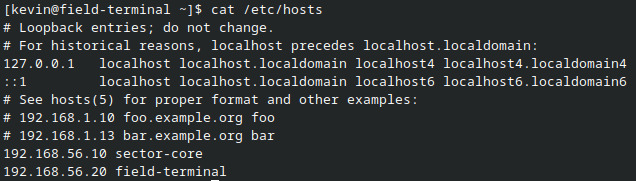
\includegraphics[width=\textwidth,height=3.8cm,keepaspectratio]{../images/etapa02_hosts_rocky.jpg}
        \caption{Archivo \texttt{/etc/hosts} en Rocky Linux (\texttt{field-terminal}): entradas para \texttt{sector-core} y \texttt{field-terminal} en la red \texttt{192.168.56.0/24}.}
        \label{fig:hosts_rocky}
    \end{subfigure}
    \hfill
    \begin{subfigure}[b]{0.48\textwidth}
        \centering
        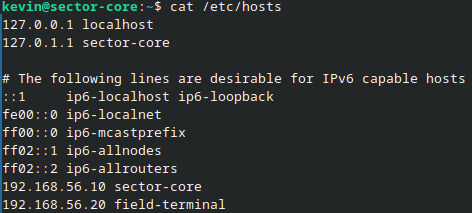
\includegraphics[width=\textwidth,height=3.8cm,keepaspectratio]{../images/etapa02_hosts_ubuntu.jpg}
        \caption{Archivo \texttt{/etc/hosts} en Ubuntu Server (\texttt{sector-core}): mismas entradas simétricas configuradas.}
        \label{fig:hosts_ubuntu}
    \end{subfigure}
    \caption{Resolución estática de nombres configurada en ambas VMs mediante \texttt{/etc/hosts}.}
    \label{fig:etapa02_hosts}
\end{figure}

\subsection{Verificación Experimental de Conectividad (ICMP Ping)}

Una vez configurada la resolución de nombres, se verifico la conectividad bidireccional en Capa 3 mediante \texttt{ping -c 3}. La prueba resuelve el nombre del destino usando \texttt{/etc/hosts} y envia 3 paquetes ICMP Echo Request, comprobando que ambas VMs se alcanzan mutuamente a través de la red interna:

\begin{itemize}[leftmargin=*]
    \item \textbf{Rocky → Ubuntu}: \texttt{ping -c 3 sector-core} desde \texttt{field-terminal} resolvió a \texttt{192.168.56.10} con \textbf{0\% packet loss} y RTT promedio de \textbf{0.768 ms}.
    \item \textbf{Ubuntu → Rocky}: \texttt{ping -c 3 field-terminal} desde \texttt{sector-core} resolvió a \texttt{192.168.56.20} con \textbf{0\% packet loss} y RTT promedio de \textbf{0.572 ms}.
\end{itemize}

\begin{figure}[H]
    \centering
    \begin{subfigure}[b]{0.48\textwidth}
        \centering
        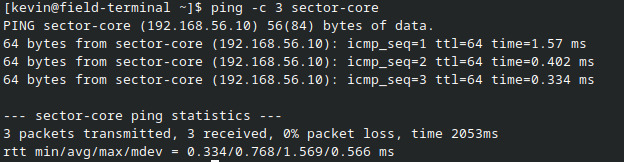
\includegraphics[width=\textwidth,height=3.8cm,keepaspectratio]{../images/etapa02_ping_rocky.jpg}
        \caption{\texttt{ping -c 3 sector-core} desde Rocky Linux: 0\% packet loss, RTT avg 0.768 ms.}
        \label{fig:ping_rocky}
    \end{subfigure}
    \hfill
    \begin{subfigure}[b]{0.48\textwidth}
        \centering
        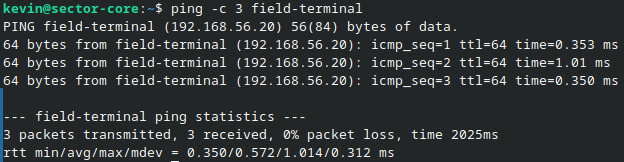
\includegraphics[width=\textwidth,height=3.8cm,keepaspectratio]{../images/etapa02_ping_ubuntu.jpg}
        \caption{\texttt{ping -c 3 field-terminal} desde Ubuntu: 0\% packet loss, RTT avg 0.572 ms.}
        \label{fig:ping_ubuntu}
    \end{subfigure}
    \caption{Verificación de conectividad bidireccional en Capa 3 entre \texttt{field-terminal} y \texttt{sector-core}.}
    \label{fig:etapa02_conectividad}
\end{figure}

% ==============================================================================
% ETAPA 03 — USUARIOS, GRUPOS Y PRIVILEGIOS
% ==============================================================================
\section{Etapa 03 — Usuarios, Grupos y Privilegios}

\subsection{Fundamentación Teórica}

\begin{pregunta}{¿Qué diferencia fundamental existe entre un usuario y un grupo?}
    \textbf{Respuesta:} Un \textbf{usuario} representa una identidad individual en el sistema asociada a un identificador entero único (\textbf{UID}). Puede representar una persona física o un demonio del sistema. Un \textbf{grupo} es una entidad colectiva identificada por un \textbf{GID}, utilizada para aplicar políticas de permisos concurrentes sobre archivos y procesos en el esquema DAC (\textit{Discretionary Access Control}).
\end{pregunta}

\begin{pregunta}{¿Qué información contienen \texttt{/etc/passwd}, \texttt{/etc/group} y \texttt{/etc/shadow}?}
    \textbf{Respuesta:}
    \begin{itemize}[leftmargin=*]
        \item \textbf{\texttt{/etc/passwd}} (permisos \texttt{644}): Registro de cuentas estructurado como \texttt{username:x:UID:GID:GECOS:home:shell}. La \texttt{x} indica que el hash de la clave se ubica en \texttt{shadow}.
        \item \textbf{\texttt{/etc/group}} (permisos \texttt{644}): Define composición de grupos: \texttt{group\_name:x:GID:user\_list}.
        \item \textbf{\texttt{/etc/shadow}} (permisos \texttt{600}): Información crítica de autenticación: \texttt{username:hash:last\_change:min:max:warn:inact:expire}. Almacena hashes con \textit{salt} (SHA-512 / Yescrypt).
    \end{itemize}
\end{pregunta}

\begin{pregunta}{¿Qué representan el UID y el GID en la arquitectura del sistema?}
    \textbf{Respuesta:} Son valores numéricos enteros utilizados por el kernel Linux en la estructura de credenciales de procesos (\texttt{struct cred}) para evaluar permisos de acceso en llamadas al sistema (\texttt{open}, \texttt{read}, \texttt{write}, \texttt{kill}).
\end{pregunta}

\begin{pregunta}{¿Qué diferencia existe entre el grupo primario y los grupos suplementarios?}
    \textbf{Respuesta:} El \textbf{grupo primario} define el GID propietario por defecto de los archivos creados por el usuario en su sesión interactiva. Los \textbf{grupos suplementarios} son membresías adicionales para acceder a recursos compartidos (como \texttt{sudo}, \texttt{wheel} o \texttt{docker}).
\end{pregunta}

\begin{pregunta}{¿Por qué el usuario root posee un tratamiento especial?}
    \textbf{Respuesta:} \texttt{root} posee el \textbf{UID = 0}. El kernel omite las comprobaciones habituales de permisos cuando el UID efectivo es 0, otorgándole acceso irrestricto sobre recursos de hardware, memoria y sistema de archivos.
\end{pregunta}

\begin{pregunta}{¿Qué problemática intenta resolver el comando \texttt{sudo}?}
    \textbf{Respuesta:} Permite ejecutar comandos privilegiados de forma granular sin divulgar la contraseña de \texttt{root}. Ofrece autenticación individual, control fino en \texttt{/etc/sudoers} y auditoría completa en los logs (\texttt{/var/log/auth.log} en Ubuntu o \texttt{/var/log/secure} en Rocky).
\end{pregunta}

\begin{pregunta}{¿Qué implica aplicar el Principio de Mínimo Privilegio (PoLP)?}
    \textbf{Respuesta:} Exige conceder a cada usuario o servicio únicamente los privilegios estrictamente necesarios para su operación, reduciendo la superficie de ataque y el impacto de errores operativos o compromisos de seguridad.
\end{pregunta}

\subsection{Configuración Aplicada}

En ambos nodos se creó la cuenta de administración individual \texttt{kevin}, asignada al grupo administrativo correspondiente a cada distribución: \texttt{wheel} en Rocky Linux (\texttt{field-terminal}) y \texttt{sudo} en Ubuntu Server (\texttt{sector-core}). Esta elección respeta el principio de mínimo privilegio: el usuario no opera como \texttt{root} en su sesión habitual, pero puede elevar privilegios cuando es necesario mediante \texttt{sudo}.

Para verificar y documentar la configuración se ejecutaron dos comandos en cada maquina:

\begin{itemize}
    \item \texttt{getent group wheel} / \texttt{getent group sudo} — consulta la base de datos de grupos del sistema (unificando \texttt{/etc/group} con fuentes NSS). Permite confirmar qué usuarios pertenecen al grupo administrativo sin editar archivos directamente.
    \item \texttt{sudo grep -E '\^{}\%wheel' /etc/sudoers} / \texttt{sudo grep -E '\^{}\%sudo' /etc/sudoers} — extrae del archivo de política \texttt{sudoers} la regla que otorga privilegios completos al grupo. La salida \texttt{\%wheel ALL=(ALL) ALL} (Rocky) y \texttt{\%sudo ALL=(ALL:ALL) ALL} (Ubuntu) confirman que cualquier miembro del grupo puede ejecutar cualquier comando como cualquier usuario, satisfaciendo los requisitos de administración delegada.
\end{itemize}

\begin{figure}[H]
    \centering
    \begin{subfigure}[b]{0.48\textwidth}
        \centering
        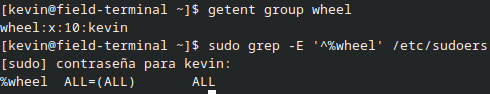
\includegraphics[width=\textwidth,height=4.0cm,keepaspectratio]{../images/etapa03_sudo_rocky.jpg}
        \caption{Verificación en Rocky Linux (\texttt{field-terminal}): \texttt{kevin} en el grupo \texttt{wheel} y regla \texttt{\%wheel ALL=(ALL) ALL} en \texttt{sudoers}.}
        \label{fig:sudo_rocky}
    \end{subfigure}
    \hfill
    \begin{subfigure}[b]{0.48\textwidth}
        \centering
        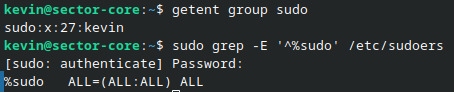
\includegraphics[width=\textwidth,height=4.0cm,keepaspectratio]{../images/etapa03_sudo_ubuntu.jpg}
        \caption{Verificación en Ubuntu Server (\texttt{sector-core}): \texttt{kevin} en el grupo \texttt{sudo} y regla \texttt{\%sudo ALL=(ALL:ALL) ALL} en \texttt{sudoers}.}
        \label{fig:sudo_ubuntu}
    \end{subfigure}
    \caption{Documentación de los usuarios con privilegios administrativos delegados en ambas distribuciones.}
    \label{fig:etapa03_sudo}
\end{figure}

% ==============================================================================
% ETAPA 04 — ACCESO REMOTO MEDIANTE SSH
% ==============================================================================
\section{Etapa 04 — Acceso Remoto Seguro mediante SSH}

\subsection{Investigación Previa}

\begin{pregunta}{¿Qué problema resuelve SSH frente a protocolos tradicionales?}
    \textbf{Respuesta:} Reemplaza protocolos no seguros (como Telnet o FTP) que transmiten credenciales y datos en texto plano. SSH-2 cifra el canal íntegro mediante algoritmos simétricos robustos (AES, ChaCha20) tras un intercambio Diffie-Hellman autenticado.
\end{pregunta}

\begin{pregunta}{¿Diferencia entre autenticación por contraseña y por clave publica?}
    \textbf{Respuesta:} La contraseña es vulnerable a fuerza bruta y viaja por el túnel cifrado hacia el servidor. En la autenticacion por clave publica, el servidor emite un desafio aleatorio (\textit{nonce}) que el cliente firma con su clave privada; la clave privada jamás abandona el equipo local.
\end{pregunta}

\begin{pregunta}{¿Función de la clave privada, clave publica y archivo \texttt{authorized\_keys}?}
    \textbf{Respuesta:} La \textbf{clave privada} firma desafíos para certificar identidad; la \textbf{clave pública} permite al servidor verificar la firma. El archivo \path{~/.ssh/authorized_keys} (permisos \texttt{600}) en el servidor almacena las claves públicas autorizadas. La clave privada nunca debe residir en el servidor para evitar escaladas laterales si el host es comprometido.
\end{pregunta}

\begin{pregunta}{¿Qué riesgo implica permitir acceso remoto directo como root?}
    \textbf{Respuesta:} Ofrece un vector fijo y predecible para ataques automatizados de fuerza bruta y anula la trazabilidad de auditoría en los registros del sistema.
\end{pregunta}

\subsection{Generación y Distribución de Claves (Ed25519)}

La consigna establece que \texttt{field-terminal} (Rocky Linux) debe poder administrar \texttt{sector-core} (Ubuntu Server) mediante SSH con autenticación por clave pública. Para ello, el par de claves se generó \textbf{dentro de la propia VM Rocky Linux}, que actúa como cliente SSH, y la clave pública fue distribuida hacia Ubuntu a través de la red interna compartida entre ambas VMs (\texttt{192.168.56.0/24}).

Desde una sesión ya iniciada en Rocky Linux se ejecutó \texttt{ssh-keygen -t ed25519}, generando el par de claves Ed25519 almacenado en \texttt{/home/kevin/.ssh/id\_ed25519} y \texttt{id\_ed25519.pub}. A continuación se usó \texttt{ssh-copy-id kevin@192.168.56.10} para registrar la clave pública en el archivo \texttt{authorized\_keys} de Ubuntu, utilizando directamente la IP interna de la red entre las VMs.

\begin{figure}[H]
    \centering
    \begin{subfigure}[b]{0.48\textwidth}
        \centering
        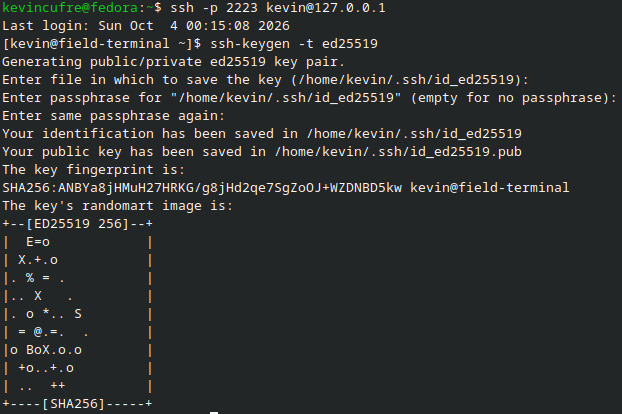
\includegraphics[width=\textwidth,height=4.0cm,keepaspectratio]{../images/etapa04_ssh_keygen_rocky.jpg}
        \caption{Generación del par de claves Ed25519 desde Rocky Linux (\texttt{field-terminal}).}
        \label{fig:ssh_keygen}
    \end{subfigure}
    \hfill
    \begin{subfigure}[b]{0.48\textwidth}
        \centering
        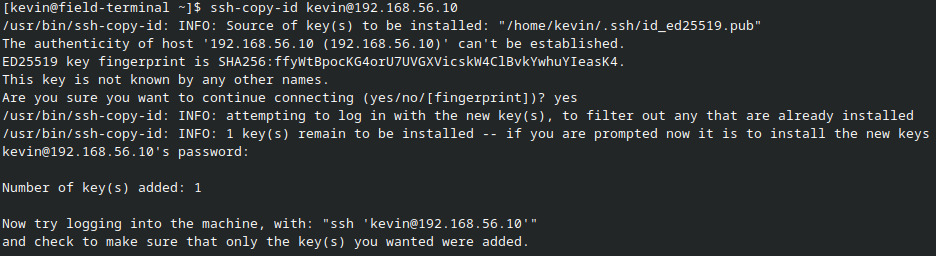
\includegraphics[width=\textwidth,height=4.0cm,keepaspectratio]{../images/etapa04_ssh_copy_id_rocky_ubuntu.jpg}
        \caption{Distribución de la clave pública a Ubuntu (\texttt{192.168.56.10}) con \texttt{ssh-copy-id}.}
        \label{fig:ssh_copy_id}
    \end{subfigure}
    \caption{Generación en Rocky y despliegue de la clave pública hacia Ubuntu a traves de la red interna de las VMs.}
    \label{fig:etapa04_ssh_setup}
\end{figure}

\subsection{Verificación de la Conexión VM a VM mediante SSH}

Una vez registrada la clave pública en Ubuntu, se verificó la conexión directa entre las VMs: desde Rocky Linux se ejecutó \texttt{ssh kevin@192.168.56.10}, estableciéndose la sesión sin requerir contraseña. La autenticación se resolvió exclusivamente mediante el par de claves Ed25519. El banner de bienvenida de Ubuntu Server confirma que la conexión fue exitosa y que \texttt{field-terminal} puede administrar \texttt{sector-core} de forma remota y segura a través de la red interna.

\begin{figure}[H]
    \centering
    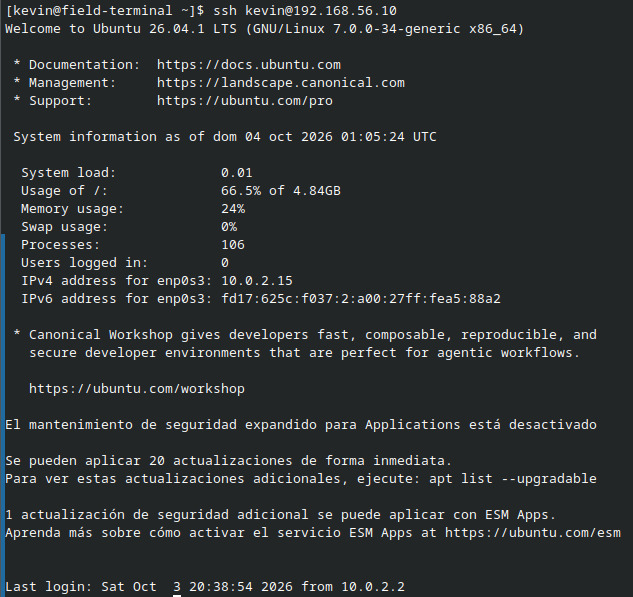
\includegraphics[width=0.85\textwidth]{../images/etapa04_ssh_conexion_verificacion.jpg}
    \caption{Conexión SSH exitosa desde Rocky Linux (\texttt{field-terminal}) hacia Ubuntu Server (\texttt{sector-core}, \texttt{192.168.56.10}) por la red interna de las VMs.}
    \label{fig:etapa04_ssh_verificacion}
\end{figure}

\subsection{Hardening: Deshabilitación del Login Remoto de Root}
En \texttt{/etc/ssh/sshd\_config} de ambos sistemas se configuró \texttt{PermitRootLogin no} y \texttt{PubkeyAuthentication yes}. Posteriormente se reiniciaron los servicios: \texttt{systemctl restart ssh} (Ubuntu) y \texttt{systemctl restart sshd} (Rocky).

\begin{figure}[H]
    \centering
    \begin{subfigure}[b]{0.48\textwidth}
        \centering
        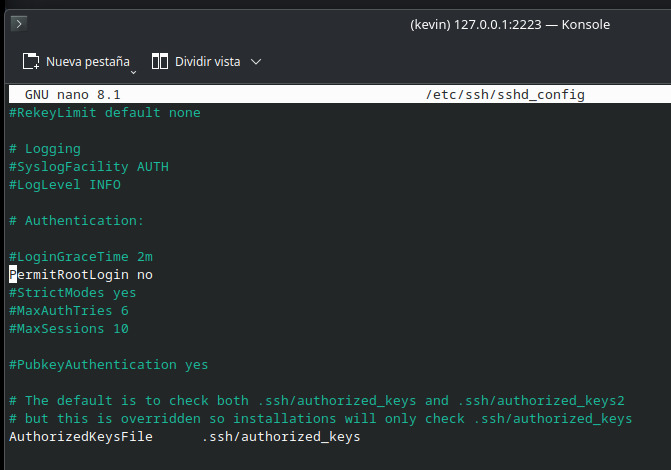
\includegraphics[width=\textwidth,height=3.8cm,keepaspectratio]{../images/etapa04_root_rocky.jpg}
        \caption{\texttt{sshd\_config} en Rocky Linux (puerto 2223).}
        \label{fig:root_rocky}
    \end{subfigure}
    \hfill
    \begin{subfigure}[b]{0.48\textwidth}
        \centering
        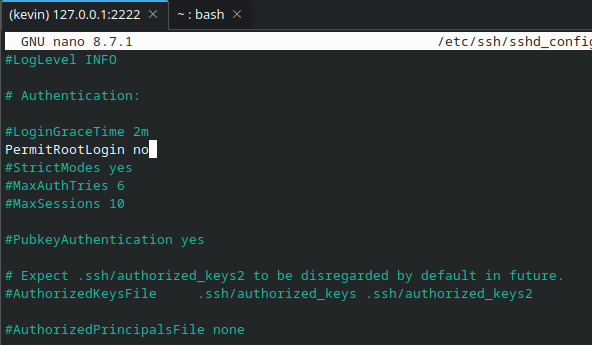
\includegraphics[width=\textwidth,height=3.8cm,keepaspectratio]{../images/etapa04_root_ubuntu.jpg}
        \caption{\texttt{sshd\_config} en Ubuntu Server (puerto 2222).}
        \label{fig:root_ubuntu}
    \end{subfigure}
    \caption{Deshabilitación de acceso remoto para \texttt{root} en ambas distribuciones.}
    \label{fig:etapa04_root_disable}
\end{figure}

% ==============================================================================
% ETAPA 05 — INVENTARIO DEL SISTEMA
% ==============================================================================
\section{Etapa 05 — Inventario Automatizado del Sistema}

\subsection{Diseño del Script y Política de Manejo de Errores}

Para cumplir con la consigna de relevamiento del sistema se desarrolló el script \texttt{system-inventory.sh} en lenguaje Bash. El script fue concebido bajo dos requerimientos primordiales: \textbf{agnosticismo respecto a la distribución} (compatibilidad plena entre Debian/Ubuntu Server y RHEL/Rocky Linux sin codificación de rutas propietarias) y \textbf{tolerancia y supervivencia ante fallos} mediante una política de control de errores.

\subsubsection{Agnosticismo de Distribución e Introspección Segura}
El script no asume utilidades ni rutas exclusivas de una única familia de sistemas operativos. En lugar de verificar archivos específicos como \texttt{/etc/debian\_version} o \texttt{/etc/redhat-release}, implementa estandares abiertos y mecanismos de introspección defensiva:
\begin{itemize}[leftmargin=*]
    \item \textbf{Estándar \texttt{/etc/os-release}}: Carga de manera controlada el archivo estándar de especificación \texttt{os-release}, extrayendo las variables \texttt{PRETTY\_NAME} y \texttt{VERSION\_ID} con mecanismos de sustitución por omisión (\texttt{\$\{PRETTY\_NAME:-desconocida\}}), complementado con las llamadas estándar POSIX \texttt{uname -r} (kernel) y \texttt{uname -m} (arquitectura).
    \item \textbf{Verificación previa de herramientas (\texttt{command\_exists})}: Mediante la función auxiliar:
    \begin{center}
    \texttt{command\_exists() \{ command -v "\$1" >/dev/null 2>\&1; \}}
    \end{center}
    se comprueba la existencia de cada binario (\texttt{lscpu}, \texttt{free}, \texttt{lsblk}, \texttt{df}, \texttt{mountpoint}, \texttt{ip}, \texttt{systemctl}) antes de su invocación. De este modo, si una utilidad no estuviera disponible en una instalación minimalista, el script notifica el error por el canal de diagnóstico estándar (\texttt{stderr}) y retorna un código de error de sección sin provocar abortos inesperados.
    \item \textbf{Procesamiento de opciones de línea de comandos}: Implementa la función \texttt{usage()} y procesa banderas mediante la primitiva \texttt{getopts ":h"}. Si se invoca con \texttt{-h}, despliega la sintaxis y ayuda finalizando limpiamente con código \texttt{EXIT\_OK} (0). Si se provee un argumento desconocido, reporta la opción inválida por \texttt{stderr}, emite la ayuda y finaliza con código de error sintáctico \texttt{EXIT\_ARGS} (1).
\end{itemize}

\subsubsection{Política de Supervivencia y Manejo de Errores (\texttt{set -euo pipefail})}
La consigna plantea una pregunta clave de ingeniería de sistemas: \textit{¿ante la falla de una consulta, el script debe continuar, detenerse o ignorar el error?}
La decisión de diseño adoptada fue la de \textbf{supervivencia con degradación informada}: ante el fallo de un componente, el script debe continuar recolectando el resto de las secciones, pues \textbf{un inventario parcial es significativamente más valioso para la administración que un script que aborta a mitad de camino sin producir resultados}. Sin embargo, el error nunca debe ser ignorado: debe registrarse en \texttt{stderr} y reflejarse en el código de salida final del proceso.

Para implementar esta política se recurre a la directiva estricta de Bash \texttt{set -euo pipefail}:
\begin{itemize}[leftmargin=*]
    \item \textbf{\texttt{-e} (\textit{errexit})}: Provoca que aborte la ejecución de una función si algún comando retorna un código distinto de 0. Para permitir que el script sobreviva entre secciones, la función principal \texttt{main()} invoca a cada bloque acoplado a un operador lógico condicional:
    \begin{center}
    \texttt{section\_os || exit\_code=1} \quad \dots \quad \texttt{section\_network || exit\_code=1}
    \end{center}
    Si una sección falla internamente, \texttt{-e} interrumpe inmediatamente dicha función (impidiendo la ejecución en cascada de comandos posteriores sobre estados corruptos), pero el operador \texttt{||} captura el estado de error, marca la variable global \texttt{exit\_code=1} y cede el control a la siguiente sección del inventario.
    \item \textbf{\texttt{-u} (\textit{nounset})}: Fuerza la terminación del script si se intenta expandir una variable que no ha sido definida previamente. Esto evita errores silenciosos producidos por fallas tipográficas en variables (ej. confundir \texttt{\$svc} con \texttt{\$srv}) o variables de entorno no inicializadas.
    \item \textbf{\texttt{-o pipefail}}: En el estándar POSIX/Bash convencional, el código de salida de un pipeline (\texttt{cmd1 | cmd2 | cmd3}) es únicamente el del último comando (\texttt{cmd3}). Bajo \texttt{pipefail}, la canalización devuelve el código del comando que falló situado más a la derecha que haya retornado distinto de cero. Esto garantiza que fallos en comandos iniciales de filtrado (como \texttt{lscpu} o \texttt{df}) no queden encubiertos por un \texttt{grep} o \texttt{sed} posterior que termine en 0.
\end{itemize}

\subsubsection{Semántica de Códigos de Salida}
El script utiliza códigos de salida normalizados y predecibles:
\begin{itemize}[leftmargin=*]
    \item \texttt{EXIT\_OK = 0}: Ejecución perfecta; todas las secciones se completaron con exito.
    \item \texttt{EXIT\_ARGS = 1}: Error en los parámetros o banderas de ejecucion.
    \item \texttt{1}: Ejecución finalizada pero con fallas o advertencias críticas registradas en una o más secciones.
    \item Enfoque \textit{best-effort} para servicios: la sección \texttt{section\_services} se ejecuta con \texttt{|| true} en \texttt{main()}, permitiendo que si el sistema carece de \texttt{systemd} (como un contenedor sin init), se reporte la limitación por \texttt{stderr} sin invalidar el inventario general del nodo.
\end{itemize}

\subsection{Análisis Funcional de las Secciones del Inventario}

El script organiza la recolección en seis módulos funcionales independientes:
\begin{enumerate}[leftmargin=*]
    \item \textbf{Sistema Operativo (\texttt{section\_os})}: Extrae distribución, version comercial, version del kernel (\texttt{uname -r}) y arquitectura (\texttt{uname -m}) a partir de \texttt{/etc/os-release}.
    \item \textbf{Procesador (\texttt{section\_cpu})}: Mediante \texttt{lscpu}, aísla las líneas de modelo, frecuencia en MHz, número de núcleos lógicos (\texttt{CPU(s)}) y núcleos por socket, complementando con la jerarquía de memoria cache (L1d, L1i, L2 y L3).
    \item \textbf{Memoria Principal y Swap (\texttt{section\_memory})}: Utiliza \texttt{free -h} para exponer en unidades legibles (MiB/GiB) la memoria RAM total, usada, libre, compartida, buffers/caché y disponible para nuevas aplicaciones, junto con el estado del espacio de intercambio (Swap).
    \item \textbf{Almacenamiento y Filesystems (\texttt{section\_storage})}: 
    \begin{itemize}
        \item Muestra los dispositivos de bloque y su particionamiento con \texttt{lsblk -o NAME,SIZE,TYPE,FSTYPE,MOUNTPOINT}.
        \item Informa la ocupación y tipos de filesystems montados con \texttt{df -hT}, excluyendo explícitamente sistemas virtuales en RAM mediante \texttt{--exclude-type=tmpfs --exclude-type=devtmpfs}.
        \item Inspecciona específicamente el punto de montaje \texttt{/mnt} mediante la utilidad \texttt{mountpoint -q /mnt}. Si detecta un sistema montado, ejecuta \texttt{df -h /mnt}; caso contrario, informa explícitamente que no hay ningún filesystem asociado, dando cumplimiento exacto a la consigna.
    \end{itemize}
    \item \textbf{Red y Conectividad (\texttt{section\_network})}: Define al comando \texttt{ip} como componente indispensable (retorna código 1 si falta). Presenta un resumen compacto de interfaces y direcciones IP con \texttt{ip -brief addr show} y lista las entradas de resolución de enlace mediante \texttt{ip neigh show}.
    \item \textbf{Servicios del Sistema (\texttt{section\_services})}: Examina una lista representativa de servicios críticos de ambas distribuciones (\texttt{sshd}, \texttt{ssh}, \texttt{NetworkManager}, \texttt{networking}, \texttt{firewalld}, \texttt{ufw}). Para cada uno determina con rigor si la unidad no existe (consultando \texttt{systemctl list-unit-files}), o su estado operativo (\texttt{active}, \texttt{inactive}, \texttt{failed}) mediante \texttt{systemctl is-active}.
\end{enumerate}

\subsection{Código Fuente Completo de \texttt{system-inventory.sh}}

A continuación se transcribe el código desarrollado en \texttt{\textasciitilde/SOI-2026-infostealer/scripts/system-inventory.sh}, presentado de forma compacta en dos columnas:

\begin{multicols*}{2}
\begin{lstlisting}[language=bash, basicstyle=\fontsize{5.2pt}{6.0pt}\ttfamily\color{darkslate}, numbers=left, numberstyle=\tiny\color{gray!70}, stepnumber=10, xleftmargin=1.0em]
#!/usr/bin/env bash
#
# system-inventory.sh - Inventario del sistema (TP1, NEXUS-9)
# system-inventory.sh
# NEXUS-9 - Script de inventario del sistema
#
# Implementación a cargo de cada grupo. El contrato que verifica CI está en
# docs/contrato-system-inventory.md.
# Agnostico de distribucion: funciona tanto en Ubuntu Server (Debian-based)
# como en Rocky Linux (RHEL-based), sin valores codificados para una
# distribución específica.

set -euo pipefail

# -- Códigos de salida ----------------------------------------------------
readonly EXIT_OK=0
readonly EXIT_ARGS=1

# -- Utilidades ------------------------------------------------------------

log_section() {
    printf '\n=== %s ===\n' "$1"
}

# Verifica si un comando existe en el sistema
command_exists() {
    command -v "$1" >/dev/null 2>&1
}

usage() {
    cat <<EOF
Uso: $(basename "$0") [-h]

Genera un inventario del sistema local: sistema operativo, CPU, memoria,
almacenamiento, red y servicios systemd.

Opciones:
  -h    Muestra esta ayuda y termina.
EOF
}

# -- Parseo de argumentos ------------------------------------------------
while getopts ":h" opt; do
    case "$opt" in
        h)
            usage
            exit "$EXIT_OK"
            ;;
        \?)
            printf 'Opción inválida: -%s\n' "$OPTARG" >&2
            usage >&2
            exit "$EXIT_ARGS"
            ;;
    esac
done

# -- Sistema operativo -----------------------------------------------------
section_os() {
    log_section "Sistema operativo"

    if [[ -r /etc/os-release ]]; then
        # shellcheck source=/dev/null
        source /etc/os-release
        printf 'Distribución : %s\n' "${PRETTY_NAME:-desconocida}"
        printf 'Versión      : %s\n' "${VERSION_ID:-desconocida}"
    else
        printf '[ERROR] No se pudo leer /etc/os-release\n' >&2
    fi

    printf 'Kernel       : %s\n' "$(uname -r)"
    printf 'Arquitectura : %s\n' "$(uname -m)"
}

# -- CPU --------------------------------------------------------------------
section_cpu() {
    log_section "CPU"

    if command_exists lscpu; then
        local modelo frecuencia cpus_logicas nucleos

        modelo=$(lscpu | grep -i '^Model name:' | sed 's/^Model name:\s*//')
        frecuencia=$(lscpu | grep -i '^CPU MHz:' | sed 's/^CPU MHz:\s*//')
        cpus_logicas=$(lscpu | grep -i '^CPU(s):' | head -1 | sed 's/^CPU(s):\s*//')
        nucleos=$(lscpu | grep -i '^Core(s) per socket:' | sed 's/^Core(s) per socket:\s*//')

        printf 'Modelo           : %s\n' "${modelo:-desconocido}"
        printf 'Frecuencia (MHz) : %s\n' "${frecuencia:-no disponible}"
        printf 'CPUs lógicas     : %s\n' "${cpus_logicas:-desconocido}"
        printf 'Cores por socket : %s\n' "${nucleos:-desconocido}"

        printf '\nCaché:\n'
        lscpu | grep -i 'cache' || printf '  No se encontró información de caché\n'
    else
        printf '[ERROR] lscpu no está disponible en este sistema\n' >&2
        return 1
    fi
}

# -- Memoria ----------------------------------------------------------------
section_memory() {
    log_section "Memoria"

    if command_exists free; then
        free -h
    else
        printf '[ERROR] free no está disponible en este sistema\n' >&2
        return 1
    fi
}

# -- Almacenamiento -------------------------------------------------------
section_storage() {
    log_section "Almacenamiento"

    printf -- '--- Dispositivos de bloque ---\n'
    if command_exists lsblk; then
        lsblk -o NAME,SIZE,TYPE,FSTYPE,MOUNTPOINT || \
            printf '[ERROR] Falló la consulta de dispositivos con lsblk\n' >&2
    else
        printf '[ERROR] lsblk no está disponible en este sistema\n' >&2
    fi

    printf '\n--- Filesystems montados y uso ---\n'
    if command_exists df; then
        df -hT --exclude-type=tmpfs --exclude-type=devtmpfs || \
            printf '[ERROR] Falló la consulta de espacio con df\n' >&2
    else
        printf '[ERROR] df no está disponible en este sistema\n' >&2
    fi

    printf '\n--- Punto de montaje /mnt ---\n'
    if mountpoint -q /mnt 2>/dev/null; then
        printf '/mnt tiene un filesystem montado:\n'
        df -h /mnt
    else
        printf '/mnt no tiene ningún filesystem montado actualmente.\n'
    fi
}

# -- Red --------------------------------------------------------------------
# El comando 'ip' es información esencial de esta sección: si no está
# disponible, la sección se considera fallida (código de salida distinto
# de 0), no solo un aviso por stderr.
section_network() {
    log_section "Red"

    if ! command_exists ip; then
        printf '[ERROR] El comando ip no esta disponible: no se puede obtener información de red\n' >&2
        return 1
    fi

    local rc=0

    printf -- '--- Interfaces y estado ---\n'
    ip -brief addr show || {
        printf '[ERROR] Falló la consulta de interfaces con ip addr\n' >&2
        rc=1
    }

    printf '\n--- Tabla de vecinos (ARP / NDP) ---\n'
    ip neigh show || printf 'No hay entradas en la tabla de vecinos actualmente.\n'

    return "$rc"
}

# -- Servicios (systemd) --------------------------------------------------
# Consulta el estado de una lista de servicios de interés y distingue
# activo / inactivo / inexistente / error de consulta. Es best-effort:
# si systemd no está disponible (p. ej. dentro de un contenedor), se
# informa pero no cambia el código de salida general del script.
section_services() {
    log_section "Servicios (systemd)"

    if ! command_exists systemctl; then
        printf '[AVISO] systemctl no está disponible en este sistema (¿contenedor sin systemd?)\n' >&2
        return 0
    fi

    local services=("sshd" "ssh" "NetworkManager" "networking" "firewalld" "ufw")
    local svc status

    for svc in "${services[@]}"; do
        if ! systemctl list-unit-files "${svc}.service" \
                --no-legend 2>/dev/null | grep -q "${svc}.service"; then
            printf '%-15s : no existe en este sistema\n' "$svc"
            continue
        fi

        status=$(systemctl is-active "${svc}.service" 2>/dev/null || true)
        if [[ -z "$status" ]]; then
            printf '[ERROR] %-15s : no se pudo consultar el estado\n' "$svc" >&2
        else
            printf '%-15s : %s\n' "$svc" "$status"
        fi
    done
}

# -- Main -------------------------------------------------------------------
main() {
    local exit_code="$EXIT_OK"

    printf 'NEXUS-9 :: Inventario del sistema\n'
    printf 'Generado el: %s\n' "$(date '+%Y-%m-%d %H:%M:%S')"
    printf 'Host: %s\n' "$(hostname)"

    section_os          || exit_code=1
    section_cpu          || exit_code=1
    section_memory        || exit_code=1
    section_storage        || exit_code=1
    section_network        || exit_code=1
    section_services        || true

    printf '\n=== Fin del inventario ===\n'

    exit "$exit_code"
}

main "$@"
\end{lstlisting}
\end{multicols*}

\subsection{Ejecución Experimental en Ambos Nodos (Ubuntu Server y Rocky Linux)}

Para ratificar empíricamente el carácter agnóstico y portable de \texttt{system-inventory.sh}, el script se ejecutó sucesivamente en \texttt{sector-core} (Ubuntu Server) y en \texttt{field-terminal} (Rocky Linux) desde sus respectivos repositorios (\texttt{\textasciitilde/SOI-2026-infostealer}).

\subsubsection{Validación en \texttt{sector-core} (Ubuntu Server)}

El relevamiento en el servidor principal confirma la captura íntegra y legible de las seis secciones en formato extendido (Figura~\ref{fig:sys_inv_ubuntu}):

\begin{figure}[H]
    \centering
    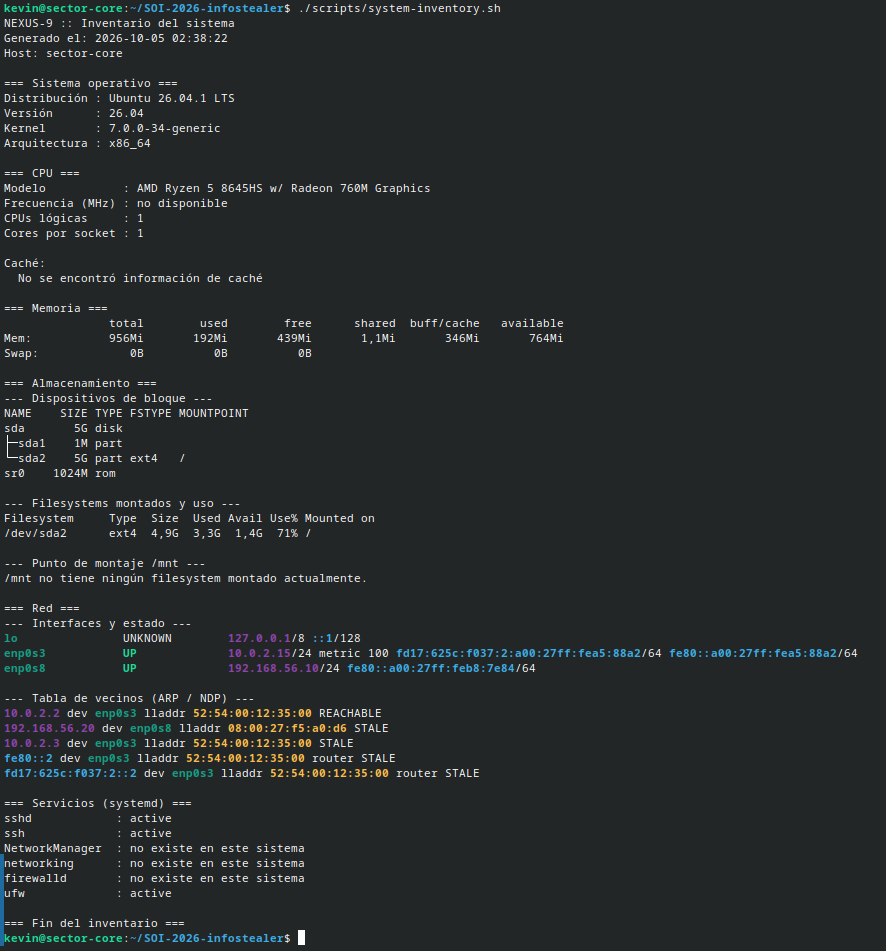
\includegraphics[width=0.94\textwidth,height=12.2cm,keepaspectratio]{../images/etapa05_system_inventory_ubuntu.png}
    \caption{Ejecución de \texttt{system-inventory.sh} en \texttt{sector-core} (Ubuntu Server 26.04.1 LTS): recolección completa de inventario bajo control de errores estricto.}
    \label{fig:sys_inv_ubuntu}
\end{figure}

\begin{itemize}[leftmargin=*, itemsep=1pt, topsep=1pt]
    \item \textbf{Sistema operativo}: Detectó correctamente \texttt{Ubuntu 26.04.1 LTS}, kernel Linux \texttt{7.0.0-34-generic} y arquitectura \texttt{x86\_64}.
    \item \textbf{CPU}: Identificó el procesador \texttt{AMD Ryzen 5 8645HS} a \texttt{4291.956 MHz}, con 1 núcleo lógico y un socket, reportando además la estructura de caché (\texttt{L1d 32 KiB}, \texttt{L1i 32 KiB}, \texttt{L2 1 MiB}, \texttt{L3 16 MiB}).
    \item \textbf{Memoria}: Se reportan \texttt{956 MiB} de RAM física total (\texttt{192 MiB} en uso, \texttt{764 MiB} utilizables). Swap de \texttt{2.0 GiB} con \texttt{0 B} de consumo.
    \item \textbf{Almacenamiento}: El comando \texttt{lsblk} refleja el disco \texttt{/dev/sda} de \texttt{25G} con partición \texttt{sda2} (\texttt{24G}, ext4 en \texttt{/}, 71\% de ocupación). Respecto a \texttt{/mnt}, confirmó que no posee ningún filesystem montado.
    \item \textbf{Red}: Reporta \texttt{lo} (\texttt{127.0.0.1/8}), \texttt{enp0s3} (\texttt{10.0.2.15/24}) y \texttt{enp0s8} (\texttt{192.168.56.10/24}).
    \item \textbf{Servicios}: Detecta activos \texttt{ssh} y \texttt{ufw}, mientras que los servicios de RHEL (\texttt{sshd}, \texttt{NetworkManager}, \texttt{firewalld}) son identificados como inexistentes sin generar error.
    \item \textbf{Código de Salida}: Concluyó exitosamente con código \texttt{0} (\texttt{echo \$? = 0}).
\end{itemize}

\clearpage
\subsubsection{Validación en \texttt{field-terminal} (Rocky Linux)}

De manera análoga, la ejecución en la terminal de campo expone en gran formato la salida adaptada a la familia Red Hat (Figura~\ref{fig:sys_inv_rocky}):

\begin{figure}[H]
    \centering
    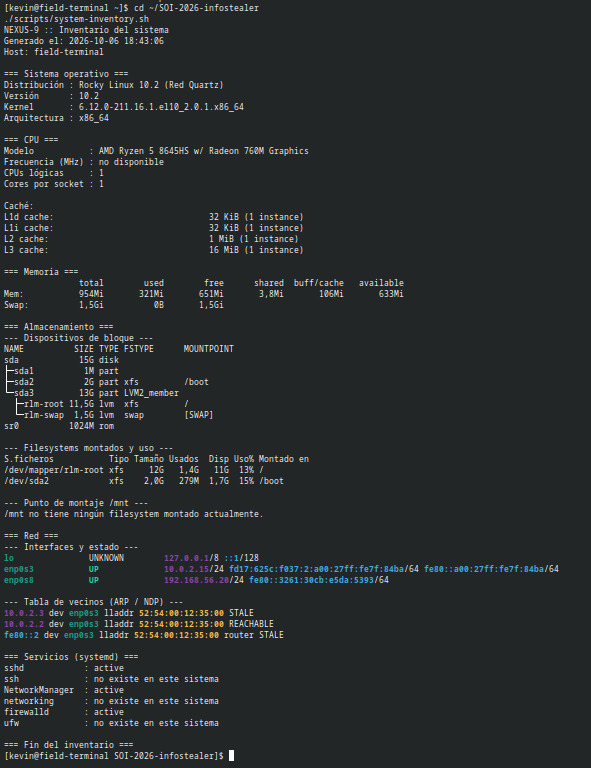
\includegraphics[width=0.94\textwidth,height=12.2cm,keepaspectratio]{../images/etapa05_system_inventory_rocky.png}
    \caption{Ejecución de \texttt{system-inventory.sh} en \texttt{field-terminal} (Rocky Linux 10.2 Red Quartz): introspección exitosa y agnóstica de hardware y servicios.}
    \label{fig:sys_inv_rocky}
\end{figure}

\begin{itemize}[leftmargin=*, itemsep=1pt, topsep=1pt]
    \item \textbf{Sistema operativo}: Leyó limpiamente \texttt{Rocky Linux 10.2 (Red Quartz)}, kernel \texttt{6.12.0-211.16.1.el10\_2.0.1.x86\_64} y arquitectura \texttt{x86\_64}.
    \item \textbf{CPU}: Identificó el mismo procesador \texttt{AMD Ryzen 5 8645HS}, 1 CPU lógica y la jerarquía de caché (L1d, L1i, L2 y L3). En la frecuencia reporta con seguridad \texttt{no disponible} al no exponerse el valor de MHz en el entorno virtual.
    \item \textbf{Memoria}: Detectó \texttt{954 MiB} de RAM física (\texttt{321 MiB} en uso, \texttt{633 MiB} disponibles) y Swap particionado de \texttt{1.5 GiB} (\texttt{0 B} usados).
    \item \textbf{Almacenamiento}: Reconoció el esquema LVM característico de RHEL con \texttt{sda} (15G) particionado en \texttt{sda2} (\texttt{xfs} en \texttt{/boot}) y \texttt{sda3} (LVM con volumen lógico \texttt{rlm-root} en \texttt{/} al 13\% de uso y \texttt{rlm-swap}). Reportó igualmente que \texttt{/mnt} no posee filesystem montado.
    \item \textbf{Red}: Expuso interfaces \texttt{lo}, \texttt{enp0s3} (\texttt{10.0.2.15/24}) y \texttt{enp0s8} (\texttt{192.168.56.20/24}). En la tabla de vecinos capturó las entradas del gateway NAT (\texttt{10.0.2.2}) y DNS (\texttt{10.0.2.3}) de VirtualBox.
    \item \textbf{Servicios}: Reflejó la correspondencia inversa a Ubuntu: identificó activos \texttt{sshd}, \texttt{NetworkManager} y \texttt{firewalld}, detectando que \texttt{ssh}, \texttt{networking} y \texttt{ufw} no existen en Rocky Linux.
    \item \textbf{Código de Salida}: En ambos entornos el script finalizó con código \texttt{0} (\texttt{echo \$? = 0}), demostrando portabilidad total y cero fallos.
\end{itemize}

\clearpage
% ==============================================================================
% ETAPA 06 — NETWORKING 101
% ==============================================================================
\section{Etapa 06 — Networking 101}

\subsection{Parte A — Identidad en la Red Local (Capa 2 vs. Capa 3)}

\begin{pregunta}{¿Qué es una dirección MAC?}
    \textbf{Respuesta:} Es un identificador unico global de hardware asignado a un controlador de interfaz de red (NIC) conforme a los estándares IEEE 802. Consta de \textbf{48 bits (6 bytes)} expresados en hexadecimal (ej. \texttt{08:00:27:f5:a0:d6}). Los primeros 24 bits corresponden al OUI (\textit{Organizationally Unique Identifier}) del fabricante y los 24 restantes son asignados unívocamente por este.
\end{pregunta}

\begin{pregunta}{¿Qué diferencias fundamentales existen entre una dirección IP y una dirección MAC? ¿En qué capa trabaja cada una?}
    \textbf{Respuesta:} La diferenciación responde al modelo de capas de la arquitectura de redes:
    
    \begin{table}[H]
        \centering
        \footnotesize
        \caption{Tabla comparativa rigurosa entre Dirección IP y Dirección MAC.}
        \label{tab:ip_vs_mac}
        \begin{tabularx}{\textwidth}{lXX}
            \toprule
            \rowcolor{tableheader}
            \textbf{Propiedad} & \textbf{Dirección IP} & \textbf{Dirección MAC} \\
            \midrule
            \textbf{Capa del Modelo OSI} & Capa 3 (Red) & Capa 2 (Enlace de Datos) \\
            \textbf{Nivel de Abstracción} & Lógica / Topológica & Física / Hardware \\
            \textbf{Ámbito de Validez} & Global e inter-redes (enrutable) & Local a un dominio de broadcast (no enrutable) \\
            \textbf{Formato y Longitud} & 32 bits (IPv4) o 128 bits (IPv6) & 48 bits (EUI-48 / 6 bytes hexadecimales) \\
            \textbf{Asignación} & Dinámica (DHCP) o estática (manual) & Quemada en ROM/firmware del NIC (BIA) \\
            \textbf{Protocolo de Asociación} & Resuelta por ARP (IPv4) o NDP (IPv6) & Origen y destino en tramas Ethernet 802.3 \\
            \bottomrule
        \end{tabularx}
    \end{table}
\end{pregunta}

\begin{pregunta}{¿La dirección MAC identifica a una computadora o a una interfaz? Si una máquina posee dos interfaces, ¿esperan encontrar una o varias MAC?}
    \textbf{Respuesta:} \textbf{Identifica a una interfaz de red específica}, no al equipo físico. Si una máquina dispone de múltiples interfaces (por ejemplo, placa Ethernet \texttt{enp0s3}, adaptador privado \texttt{enp0s8} y placa Wi-Fi), \textbf{posee una dirección MAC distinta e independiente para cada una}.
\end{pregunta}

% ------------------------------------------------------------------------------
% PARTE B — TABLA DE VECINOS
% ------------------------------------------------------------------------------
\subsection{Parte B — Tabla de Vecinos}

\begin{pregunta}{¿Qué información muestra el comando \texttt{ip neigh}?}
    \textbf{Respuesta:} Muestra la caché de vecinos de Capa 2 del kernel Linux (tabla ARP en IPv4 y NDP en IPv6). Para cada entrada conocida expone: dirección IP del vecino, interfaz local (\texttt{dev}), dirección MAC física (\texttt{lladdr}) y estado de alcanzabilidad en el kernel.
\end{pregunta}

\subsubsection{Inspección e Identificación de Entradas de Vecinos}
La inspección de las capturas obtenidas en el laboratorio revela con exactitud los dispositivos del entorno:

\begin{figure}[H]
    \centering
    \begin{subfigure}[b]{0.48\textwidth}
        \centering
        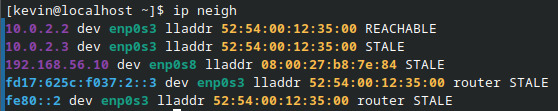
\includegraphics[width=\textwidth,height=2.9cm,keepaspectratio]{../images/etapa06_pto8_neigh_rocky.jpg}
        \caption{Tabla de vecinos en Rocky Linux (\texttt{field-terminal}).}
        \label{fig:neigh_rocky}
    \end{subfigure}
    \hfill
    \begin{subfigure}[b]{0.48\textwidth}
        \centering
        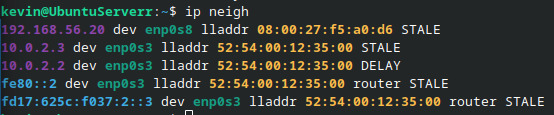
\includegraphics[width=\textwidth,height=2.9cm,keepaspectratio]{../images/etapa06_pto8_neigh_ubuntu.jpg}
        \caption{Tabla de vecinos en Ubuntu Server (\texttt{sector-core}).}
        \label{fig:neigh_ubuntu}
    \end{subfigure}
    \caption{Visualización de tablas de vecinos mediante \texttt{ip neigh} en ambos nodos.}
    \label{fig:neigh_ambos}
\end{figure}

\begin{itemize}[leftmargin=*]
    \item \textbf{En Rocky Linux (\texttt{field-terminal})}:
    \begin{itemize}
        \item \texttt{192.168.56.10 dev enp0s8 lladdr 08:00:27:b8:7e:84 STALE}: Corresponde a la interfaz privada del servidor \textbf{\texttt{sector-core}} (Ubuntu Server) en la red \texttt{192.168.56.0/24}.
        \item \texttt{10.0.2.2 dev enp0s3 lladdr 52:54:00:12:35:00 REACHABLE}: Gateway NAT del hipervisor VirtualBox.
        \item \texttt{10.0.2.3 dev enp0s3}: Servidor DNS interno provisto por VirtualBox.
        \item Entradas IPv6 (\texttt{fd17:...}, \texttt{fe80::2}) con flag \texttt{router STALE}: Descubrimiento de vecinos por NDP.
    \end{itemize}
    \item \textbf{En Ubuntu Server (\texttt{sector-core})}:
    \begin{itemize}
        \item \texttt{192.168.56.20 dev enp0s8 lladdr 08:00:27:f5:a0:d6 STALE}: Corresponde a la interfaz privada de la terminal \textbf{\texttt{field-terminal}} (Rocky Linux).
        \item \texttt{10.0.2.2 dev enp0s3 DELAY}: Gateway NAT en proceso de verificación de alcanzabilidad.
    \end{itemize}
\end{itemize}

\subsubsection{Significado de los Estados del Kernel en la Tabla de Vecinos}
\begin{table}[H]
    \centering
    \footnotesize
    \caption{Estados del autómata de vecinos en el subsistema de red de Linux (RFC 4861).}
    \label{tab:estados_arp}
    \begin{tabularx}{\textwidth}{lX}
        \toprule
        \rowcolor{tableheader}
        \textbf{Estado} & \textbf{Descripción y Comportamiento del Kernel} \\
        \midrule
        \textbf{\texttt{REACHABLE}} & Entrada confirmada y válida recientemente (confirmación bidireccional positiva). \\
        \rowcolor{rowalt}
        \textbf{\texttt{STALE}} & Validez temporal caducada por inactividad. El kernel conserva la MAC, pero revalidará con el próximo tráfico. \\
        \textbf{\texttt{DELAY}} & Se envió tráfico a una entrada en \texttt{STALE}; el kernel espera confirmación breve antes de enviar sondeos. \\
        \rowcolor{rowalt}
        \textbf{\texttt{PROBE}} & Sin confirmación en \texttt{DELAY}; el kernel emite solicitudes ARP unicast directas para verificar al vecino. \\
        \textbf{\texttt{FAILED}} & El vecino no respondió a los sondeos de solicitud ARP; la IP se marca como inalcanzable. \\
        \rowcolor{rowalt}
        \textbf{\texttt{PERMANENT}} & Entrada estática fijada manualmente (ej. con \texttt{ip neigh replace}); nunca caduca por tiempo. \\
        \bottomrule
    \end{tabularx}
\end{table}

\subsubsection{Dinámica ARP: Eliminación de Entrada y Regeneración de Tráfico}
Para comprobar el ciclo de vida de la tabla de vecinos y verificar experimentalmente qué ocurre al eliminar una entrada de forma controlada y volver a emitir tráfico, se ejecutaron las siguientes dos fases:

\paragraph{Fase 1: Vaciado y Reconstrucción Dinámica de la Tabla ARP.}
\begin{enumerate}[leftmargin=*]
    \item \textbf{Vaciado controlado de caché}: Se purgó la tabla de vecinos con \texttt{sudo ip neigh flush all}. Al volver a consultar con \texttt{ip neigh}, la entrada de la VM vecina desapareció por completo de la memoria del kernel.
    \item \textbf{Generación de nuevo tráfico}: Se disparó un paquete ICMP con \texttt{ping -c 1 192.168.56.20}. El kernel detectó la ausencia de la entrada ARP para dicha IP en \texttt{enp0s8}, retuvo temporalmente el datagrama en buffer y transmitió un \textbf{ARP Request} en broadcast (\texttt{FF:FF:FF:FF:FF:FF}).
    \item \textbf{Respuesta y Reaprendizaje}: El host \texttt{field-terminal} respondió con un \textbf{ARP Reply} unicast informando su dirección MAC física (\texttt{08:00:27:f5:a0:d6}). El kernel local reinstaló automáticamente la entrada en estado \textbf{\texttt{REACHABLE}} y transmitió el ping con éxito (0\% de pérdida).
\end{enumerate}

\paragraph{Fase 2: Inyección de Entrada Corrupta (Conflicto de MAC).}
Para corroborar la dependencia absoluta de Capa 3 respecto de Capa 2, se fijó una MAC inexistente:
\begin{lstlisting}[language=bash]
sudo ip neigh replace 192.168.56.20 lladdr aa:bb:cc:dd:ee:ff dev enp0s8
\end{lstlisting}
El registro pasó a estado estático \textbf{\texttt{PERMANENT}}. Al reintentar la comunicación con \texttt{ping -c 2 192.168.56.20}, se produjo un \textbf{100\% de pérdida de paquetes}. El emisor encapsuló los datagramas IP dentro de tramas Ethernet dirigidas a la MAC falsa; como ningún NIC de la red poseía dicha dirección física, las tramas fueron descartadas a nivel de enlace de hardware. Esto ratifica que una IP válida en Capa 3 es inútil si la correspondencia ARP en Capa 2 es inconsistente.

\begin{figure}[H]
    \centering
    \begin{subfigure}[b]{0.48\textwidth}
        \centering
        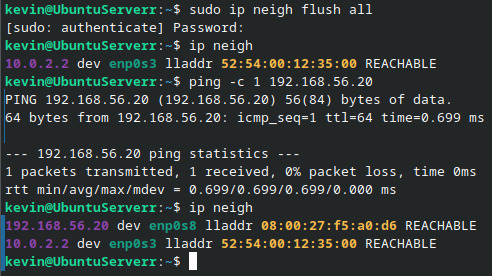
\includegraphics[width=\textwidth,height=3.3cm,keepaspectratio]{../images/etapa06_pto9_secuencia.jpg}
        \caption{Secuencia completa de purga, tráfico y reconstrucción.}
        \label{fig:p9_secuencia}
    \end{subfigure}
    \hfill
    \begin{subfigure}[b]{0.48\textwidth}
        \centering
        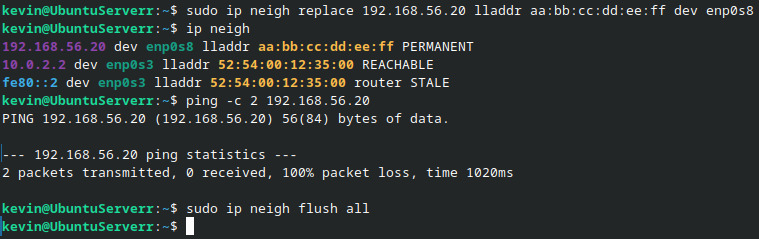
\includegraphics[width=\textwidth,height=3.3cm,keepaspectratio]{../images/etapa06_pto9_conflicto.jpg}
        \caption{Inyección de MAC falsa y fallo de comunicación (100\% loss).}
        \label{fig:p9_conflicto}
    \end{subfigure}
    \caption{Validación experimental del ciclo de vida y dinámica ARP en el sector NEXUS-9.}
    \label{fig:etapa06_arp_experimentos}
\end{figure}

% ------------------------------------------------------------------------------
% PARTE C — DOS MÁQUINAS Y UN SWITCH (SIN ROUTER)
% ------------------------------------------------------------------------------
\subsection{Parte C — Dos Máquinas y un Switch (Sin Router)}

Se analiza formalmente el siguiente escenario de interconexion fisica:

\begin{center}
\begin{tikzpicture}[node distance=1.7cm, auto, >=stealth']
    \node [rectangle, draw=uncblue, fill=boxbg, thick, rounded corners, minimum width=2.8cm, minimum height=1.1cm, align=center] (hostA) {\textbf{Máquina A}\\\scriptsize IP: $192.168.1.10/24$\\\tiny MAC: $M_A$};
    \node [rectangle, draw=accentteal, fill=tableheader, thick, minimum width=2.4cm, minimum height=1.1cm, right=of hostA, align=center] (switch) {\textbf{Switch L2}\\\scriptsize (Conmutador L2)};
    \node [rectangle, draw=uncblue, fill=boxbg, thick, rounded corners, minimum width=2.8cm, minimum height=1.1cm, right=of switch, align=center] (hostB) {\textbf{Máquina B}\\\scriptsize IP: $192.168.1.20/24$\\\tiny MAC: $M_B$};
    
    \draw [thick, <->] (hostA) -- node[above] {\scriptsize Puerto 1} (switch);
    \draw [thick, <->] (switch) -- node[above] {\scriptsize Puerto 2} (hostB);
\end{tikzpicture}
\end{center}

\begin{pregunta}{¿Pueden comunicarse dos máquinas conectadas a un switch sin router?}
    \textbf{Respuesta:} \textbf{Sí.} Dos equipos conectados a un switch en el mismo dominio de broadcast se comunican perfectamente siempre que pertenezcan a la misma subred lógica IP. El switch conmutará las tramas basándose en las direcciones MAC resueltas localmente por ARP.
\end{pregunta}

\begin{pregunta}{¿Qué condiciones deben cumplir sus direcciones IP?}
    \textbf{Respuesta:} Deben compartir la misma porción de red (definida por la máscara de subred, ej. \texttt{192.168.1.0/24}), tener Host IDs únicos para evitar colisiones y máscaras coherentes para reconocer el destino como local (\textit{on-link}).
\end{pregunta}

\begin{pregunta}{¿Qué funcion cumple exactamente el switch?}
    \textbf{Respuesta:} Opera en la \textbf{Capa 2 del modelo OSI}. Aprende dinámicamente las direcciones MAC asociándolas a sus puertos físicos en la tabla CAM, realiza reenvío selectivo unicast hacia el puerto destino correspondiente y distribuye por inundación (\textit{flooding}) únicamente tramas broadcast o con MAC destino desconocida.
\end{pregunta}

\begin{pregunta}{¿Necesitan gateway configurado para comunicarse entre ellas?}
    \textbf{Respuesta:} \textbf{No.} El gateway solo es requerido para alcanzar redes remotas o Internet. Para tráfico local, la pila TCP/IP determina que la IP destino está en el mismo enlace físico y resuelve la MAC directamente por ARP sin invocar a la puerta de enlace.
\end{pregunta}

\begin{pregunta}{¿Qué sucede si pertenecen a redes IP diferentes (ej. 192.168.1.10/24 y 10.0.0.20/24)?}
    \textbf{Respuesta:} \textbf{No pueden comunicarse directamente.} Al evaluar la máscara, el emisor determina que el destino es remoto e intenta derivar el paquete a su gateway. Si no existe gateway configurado, el kernel aborta con el error \texttt{Network is unreachable}. Si lo tiene pero no hay router físico, los paquetes se pierden. Los hosts locales no responden solicitudes ARP de subredes ajenas.
\end{pregunta}

\begin{pregunta}{¿Puede un switch convencional resolver ese escenario?}
    \textbf{Respuesta:} \textbf{No.} Un switch L2 conmuta exclusivamente tramas Ethernet basándose en direcciones MAC y no interpreta direcciones IP, máscaras ni tablas de enrutamiento.
\end{pregunta}

\begin{pregunta}{¿Qué componente sería necesario?}
    \textbf{Respuesta:} Un dispositivo de \textbf{Capa 3 (Capa de Red)}: un \textbf{Router} o un \textbf{Switch de Capa 3 (Multilayer Switch)} con enrutamiento intervlan activado.
\end{pregunta}

% ------------------------------------------------------------------------------
% COMPARATIVA DE ADMINISTRACIÓN ENTRE DISTRIBUCIONES
% ------------------------------------------------------------------------------
\subsection{Comparativa de Administración entre Distribuciones}

Durante la puesta a punto y operación de ambas máquinas virtuales se registraron divergencias arquitectónicas entre las familias Debian (Ubuntu Server) y RHEL (Rocky Linux):

\begin{table}[H]
    \centering
    \footnotesize
    \caption{Divergencias operativas prácticas entre Ubuntu Server y Rocky Linux.}
    \label{tab:comparativa_distros}
    \begin{tabularx}{\textwidth}{lXX}
        \toprule
        \rowcolor{tableheader}
        \textbf{Categoría de Administración} & \textbf{Ubuntu Server (\texttt{sector-core})} & \textbf{Rocky Linux (\texttt{field-terminal})} \\
        \midrule
        \textbf{Configuración de Red} & Utiliza \textbf{Netplan} mediante edición declarativa de archivos YAML (\texttt{/etc/netplan/*.yaml}) procesados hacia \texttt{systemd-networkd}. & Utiliza \textbf{NetworkManager} administrado mediante comandos de consola interactivos \texttt{nmcli} o archivos en \texttt{/etc/NetworkManager/}. \\
        \rowcolor{rowalt}
        \textbf{Gestión de Paquetes} & Emplea el ecosistema \textbf{APT} (\texttt{apt}, \texttt{apt-get}) con paquetes binarios en formato \texttt{.deb}. & Emplea el gestor \textbf{DNF} (\textit{Dandified YUM}) con paquetes binarios en formato \texttt{.rpm}. \\
        \textbf{Paquetes Base (Mínimo)} & Incluye utilidades comunes como el editor de texto \texttt{nano} preinstalado por defecto. & Instalación minimalista estricta; requirió instalación manual (\texttt{sudo dnf install nano}). \\
        \rowcolor{rowalt}
        \textbf{Nomenclatura de Servicios} & El servicio del demonio OpenSSH se denomina canónicamente \textbf{\texttt{ssh}} (\texttt{systemctl restart ssh}). & El servicio del demonio OpenSSH conserva el nombre del binario: \textbf{\texttt{sshd}} (\texttt{systemctl restart sshd}). \\
        \bottomrule
    \end{tabularx}
\end{table}

% ==============================================================================
% CONCLUSIONES TÉCNICAS
% ==============================================================================
\section{Conclusiones Técnicas}

La implementación integral del Trabajo Práctico N$^\circ$ 1: \textbf{“Activación del Sector NEXUS-9”} permitió articular de manera práctica y rigurosa los conceptos fundamentales de sistemas operativos, administración avanzada de entornos GNU/Linux y redes de datos:

\begin{enumerate}[leftmargin=*, itemsep=1.2pt, topsep=1.5pt]
    \item \textbf{Interoperabilidad y Arquitecturas Heterogéneas}: La coexistencia de dos familias mayores del ecosistema GNU/Linux —Debian (Ubuntu Server 26.04) y Red Hat (Rocky Linux 9)— demostró que, a pesar de sus divergencias en herramientas de configuración (Netplan declarativo frente al comando imperativo \texttt{nmcli} de NetworkManager) y gestores de paquetes (\texttt{apt} frente a \texttt{dnf}), los estándares abiertos (POSIX, \texttt{/etc/os-release}, convención FHS y subsistema del kernel) proveen un marco unificado, predecible y robusto para la operación multiplataforma.
    
    \item \textbf{Seguridad Defensiva y Mínimo Privilegio}: El diseño de privilegios jerárquicos mediante \texttt{sudo} y el aislamiento de credenciales confirmó la importancia crítica de aplicar el \textit{Principio de Mínimo Privilegio}. La configuración y endurecimiento del demonio SSH —restringiendo el acceso exclusivo a pares de llaves criptográficas asimétricas modernas \textbf{Ed25519} y deshabilitando de raíz la autenticación del superusuario \texttt{root}— neutralizan los vectores de ataque más comunes en infraestructuras expuestas, garantizando trazabilidad y confidencialidad.

    \item \textbf{Automatización Resiliente e Introspección}: El desarrollo del script \texttt{system-inventory.sh} ilustró la relevancia de adoptar políticas de diseño defensivas. La incorporación consciente de la directiva estricta \texttt{set -euo pipefail}, combinada con mecanismos de degradación controlada e introspección modular, ratificó que un proceso de auditoría debe ser capaz de sobrevivir a fallos locales para proveer información diagnóstica útil, sin silenciar los errores operacionales.

    \item \textbf{Interdependencia de Capas y Dinámica ARP}: Las pruebas experimentales sobre el subsistema de red evidenciaron la frontera indivisible entre el direccionamiento lógico (Capa 3 - IP) y la entrega física en el enlace local (Capa 2 - Ethernet). Se constató empíricamente cómo el protocolo ARP actúa como el puente indispensable en dominios de difusión locales; y cómo la alteración o desactualización de las tablas de vecinos del kernel invalida por completo el enrutamiento y la conectividad IP, corroborando el principio teórico de que la alcanzabilidad lógica depende inexorablemente de la integridad de Capa 2.
\end{enumerate}

\vspace{0.15cm}
\begin{center}
\begin{tcolorbox}[colback=uncblue!10,colframe=uncblue,width=0.88\textwidth,arc=2.5mm,center]
    \centering\bfseries\small\color{uncblue}
    SECTOR NEXUS-9: ACTIVO Y VERIFICADO OPERACIONALMENTE\\
    \footnotesize Infraestructura, Seguridad, Automatización y Networking Validados al 100\%
\end{tcolorbox}
\end{center}

\end{document}
